%%%%%%%%%%%%%%%%%%%%%%%%%%%%%%%%%%%%%%%%%
% University/School Laboratory Report
% LaTeX Template
% Version 3.0 (4/2/13)
%
% This template has been downloaded from:
% http://www.LaTeXTemplates.com
%
% Original author:
% Linux and Unix Users Group at Virginia Tech Wiki 
% (https://vtluug.org/wiki/Example_LaTeX_chem_lab_report)
%
% License:
% CC BY-NC-SA 3.0 (http://creativecommons.org/licenses/by-nc-sa/3.0/)
%
%%%%%%%%%%%%%%%%%%%%%%%%%%%%%%%%%%%%%%%%%

%----------------------------------------------------------------------------------------
%	PACKAGES AND DOCUMENT CONFIGURATIONS
%----------------------------------------------------------------------------------------

\documentclass{article}

\usepackage[version=3]{mhchem} % Package for chemical equation typesetting
\usepackage{siunitx} % Provides the \SI{}{} command for typesetting SI units

\usepackage{graphicx} % Required for the inclusion of images

\usepackage{hyperref}

\setlength\parindent{0pt} % Removes all indentation from paragraphs

\renewcommand{\labelenumi}{\alph{enumi}.} % Make numbering in the enumerate environment by letter rather than number (e.g. section 6)

%\usepackage{times} % Uncomment to use the Times New Roman font

%----------------------------------------------------------------------------------------
%	DOCUMENT INFORMATION
%----------------------------------------------------------------------------------------

\title{Bayesian networks in R with RUnBBayes package} % Title

%\author{John \textsc{Smith}} % Author name

\date{\today} % Date for the report

\begin{document}

\maketitle % Insert the title, author and date

\begin{center}
\begin{tabular}{l r}
Developers: & Fernando Santos \\ % Partner names
& Yuri Lavinas \\
& Samuel Pala \\
& Diego Marques \\
& Pedro Henrique \\
Instructor: & Rommel Carvalho % Instructor/supervisor
\end{tabular}
\end{center}

% If you wish to include an abstract, uncomment the lines below
% \begin{abstract}
% Abstract text
% \end{abstract}

%----------------------------------------------------------------------------------------
%	SECTION 1
%----------------------------------------------------------------------------------------

\section{Introduction}

The RUnBBayes package provides access to some functionalities of the UnBBayes framework. UnBBayes (\url {http://unbbayes.sourceforge.net/}) is an open source software for modeling, learning and reasoning upon probabilistic networks developed in Java. Making use of rJava, this package provides an interface to implement probabilistic networks within R.

% If you have more than one objective, uncomment the below:
%\begin{description}
%\item[First Objective] \hfill \\
%Objective 1 text
%\item[Second Objective] \hfill \\
%Objective 2 text
%\end{description}



\section{The chest clinic example}

This section explains how to use RUnBBayes in the chest clinic example of Lauritzen and Spiegelhalter (1988) (Figure~\ref{fig:asia}). As stated by Lauritzen and Spiegelhalter (1988):

\begin{quotation}
Shortness-of-breath (dyspnoea) may be due to tuberculosis, lung cancer or bronchitis, or none of them, or more than one of them. A recent visit to Asia increases the chances of tuberculosis, while smoking is known to be a risk factor for both lung cancer and bronchitis. The results of a single chest X-ray do not discriminate between lung cancer and tuberculosis, as neither does the presence or absence of dyspnoea.
\end{quotation}

\begin{figure}[ht!]
\centering
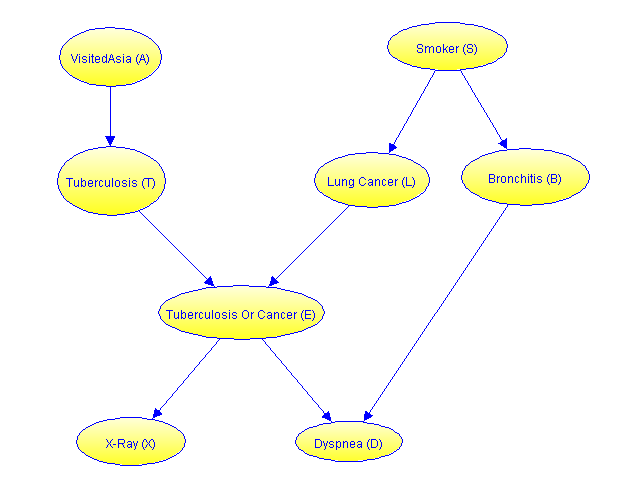
\includegraphics[width=90mm]{chest-clinic.png}
\caption{Chest clinic example}
\label{fig:asia}
\end{figure}


\subsection{Defining the network nodes}

We can create a network by defining its nodes, together with their conditional probabilities and their state. 

\begin{verbatim}
> node.a = createNodeInfo(~asia, prob=c(0.01, 0.99), states=c("yes","no"))
> node.t = createNodeInfo(~tub|asia, prob=c(0.05, 0.95, 0.01, 0.99),states=c("yes","no"))
> node.s = createNodeInfo(~smoke, prob=c(5,5), states=c("yes","no"))
> node.l = createNodeInfo(~lung|smoke, prob=c(0.1, 0.9, 0.01, 0.99), states=c("yes","no"))
> node.b = createNodeInfo(~bronc|smoke, prob=c(0.6, 0. 4, 0.3, 0.7), states=c("yes","no"))
> node.e = createNodeInfo(~either|lung:tub,prob=c(1,0,1,0,1,0,0,1),states=c("yes","no"))
> node.x = createNodeInfo(~xray|either, prob=c(0.98, 0.02, 0.05, 0.95), 
states=c("yes","no"))
> node.d = createNodeInfo(~dysp|bronc:either, prob=c(0.9, 0.1, 0.7, 0.3, 0.8, 0.2, 0.1, 
0.9), states=c("yes","no"))
\end{verbatim}


Each of these calls will return a "nodeinfo" structure.

\begin{verbatim}
> node.a = createNodeInfo(~asia, prob=c(0.01, 0.99), states=c("yes","no"))
> node.a
Node:           asia
Parents:        NA
Probabilities:  0.01, 0.99
States:         yes, no
\end{verbatim}



\subsection{Compiling the network}
Create a probabilistic newtork, from a node list.
Compile list of conditional probability tables and create the network
\begin{verbatim}
> nodeList = list(node.a, node.t, node.s, node.l, node.b, node.e, node.x, node.d)
> network = createNetwork(nodeList, compile=TRUE)

> network
Compiled: TRUE
P ( asia )
P ( tub | asia )
P ( smoke )
P ( lung | smoke )
P ( bronc | smoke )
P ( either | lungtub )
P ( xray | either )
P ( dysp | bronceither )

Setting compile as true, gives you a compiled network. Otherwise, the network won't
be compiled by default.So, it's necessary to use the compileNetwork function as an
option to build the junction tree.
> netCompiled = compileNetwork(network)
\end{verbatim}

\subsection{Querying the network}

1. The network can be queried to return the priori probabilities of all nodes:

\begin{verbatim}
> prioriProb = queryNetwork(net)
> prioriProb
$xray
		yes		no
		0.11		0.89

$bronc
		yes		no
		0.45		0.55

$dysp
		yes		no
		0.44		0.56

$asia
		yes		no
		0.01		0.99

$smoke
		yes		no
		0.5		0.5

$lung
		yes		no
		0.06		0.94

$tub
		yes		no
		0.01		0.99

$either
		yes		no
		0.06		0.94
> prioriProb$xray
$yes

		0.11

$no

		0.89

> prioriProb$xray$yes
[1] 0.11
\end{verbatim}


2. The network can be queried to return the priori probabilities of some specific nodes:

\begin{verbatim}
> prioriProb = queryNetwork(net, list(c("T", "yes"), c("L", "no")))
> prioriProb
$L
		no
		0.94

$T
		yes
		0.01
\end{verbatim}


3. The network can return the posteriori probabilities of some event given some evidences without modifying the current network object:

\begin{verbatim}
> posterioriProb = queryNetworkWithEvidences(net, c("either", "yes"), list(c("asia",
"yes"), c("smoker","no")))
> posterioriProb
$either
		yes
		0.06
\end{verbatim}


4. Evidences can be set and reset in the network:

\begin{verbatim}
> net = setEvidence(net, list(c("asia", "yes"), c("smoker", "no")))
> net = propagateEvidences(net)
> posterioriProb = queryNetwork(net, c("dysp", "yes"))
> posterioriProb
$dysp
		yes
		0.34

> net = resetEvidences(net)
> prioriProb = queryNetwork(net, c("dysp", "yes"))
> prioriProb
$dysp
		yes
		0.44

\end{verbatim}


\subsection{Updating the network}

1. Nodes can be added or removed from a compiled network:

\begin{verbatim}
> net = addNode(net, ~asthma|smoker, prob = c(0.6, 0.4, 0.85, 0.15), states = c("yes",
"no"))
> net = removeNode(net, "asthma")
\end{verbatim}










%----------------------------------------------------------------------------------------
%	BIBLIOGRAPHY
%----------------------------------------------------------------------------------------

\bibliographystyle{unsrt}

\bibliography{sample}

%----------------------------------------------------------------------------------------


\end{document}